\section{GA Outputs}
Some of the performed test runs are presented in this section. Presented outputs must be considered as examples of common algorithm behavior. Only different results were obtained by running the GA with constant settings. If not stated different, tests ran under conditions defined in section "Settings" with using the previously specified "Model Room". The axis symmetry was preferred because their outputs look better. Only fitness function (\ref{eq:fitV2EUB}) was used. In most of the tests illuminance and uniformity were considered equally important, therefore the preference factor $\alpha$ was set to $0.5$.

\subsection{Settings}

All GA settings are summarized in Table~\ref{tab:GAsettings}. All tests ended after reaching the 25\textsuperscript{th} generation. The best solution from each generation was saved in two specimens. The first specimen became a member of the next generation without mutation, i.e. the best chromosome has been passed to future generations without change. This method is called "Elitism". The second specimen was allowed to mutate with defined a probability and its purpose was to try to change the best chromosome a little.

Other parent solutions for the recombination and mutation were taken by tournament selections. A single tournament selection picked a random group of four solutions and took the one with the best fitness (minimum). This method avoided a premature convergence of the best solution. It was desirable to support diversity among solutions at least in early populations. The crossovers were made only in one point and its probability was set to~$90 \%$.

\begin{table}[htb]
	\renewcommand{\arraystretch}{1.3}
	\caption{Genetic Algorithm Settings}
 	\label{tab:GAsettings}
	\centering
  \begin{tabular}{| l | c |}
    \hline
    \textbf{First Population} & Random logic vectors \\
    \hline
    \textbf{Termination Cond.} & Defined count of generations \\
    \hline
		\textbf{Count of Gen.} & $25$ \\
    \hline
		\textbf{Population Size} & $100$ \\
	\hline
		\textbf{Parent Selection} & Tournament 1 of 4 \\
    \hline
		\textbf{Survival Selection} & Elitism \\
	\hline
		\textbf{Recombination Type} & One point \\
    \hline
		\textbf{Recombination Prob.} & $90 \%$ \\
	\hline
		\textbf{Mutation Method} & Bit inversion \& Permutation\\
	\hline
		\textbf{Mutation Prob.} & $1 \%$ \\
	\hline
		& $10 \% \left( perm. \geq 1\right)$\\
		\textbf{Permutation Prob.} &  $0.349 \% \left( perm. \geq 2\right)$ \\
		&$0.004 \% \left( perm. = 3\right)$\\
    \hline
  \end{tabular}
\end{table}

\subsection{Symmetry Comparison}

The results for both types of symmetry are presented in Figures~\ref{fig:V010_S0}, \ref{fig:V010_S1} and Table~\ref{tab:symmetry}. Mirror symmetry has a nicer look from the human's point of view, it is more common for luminaire placement so it was further preferred. There are also smaller differences among several GA outputs with identical settings.

Both symmetries have the same count of luminaires and very close resulting values. It can be said, that the resulting values are almost independent on the type of symmetry. However by using rotational symmetry the GA had more freedom placing the luminaires so its design in some cases (other room dimensions, other luminous intensity distribution curve etc.) consisted of 2 luminaries less than by using mirror symmetry. In cases where the optimal count of luminaires was the same, there were negligible result dependencies on the type of symmetry.

The rotational symmetry luminaire placement in Figure~\ref{fig:V010_S0} seems to be X shaped. That was very common during the tests. The target ratio R was set to 1 in the presented outputs. However the resulting ratio is about 0.8 in both cases of symmetry. It means that the increase of uniformity was cheaper than the increase of average illuminance. This phenomenon is dependent on the shape of the luminous intensity distribution curve. For other curves the resulting ratio would be different.

\begin{table}[tb]
	\renewcommand{\arraystretch}{1.8}
	\caption{Results for symmetry comparison}
 	\label{tab:symmetry}
	\centering
  \begin{tabular}{| c | c | c |}
    \hline
    & \textbf{Rotational symmetry} & \textbf{Mirror symmetry} \\
    \hline
    $\overline{E}_{m}$ (lx) & 501 & 506 \\
    \hline
		$U_0$ ($-$)& 0.74 & 0.74 \\
    \hline
		$C$ (-) & 16 & 16 \\
	\hline
		$R$ (-) & 0.80 & 0.82 \\
  \hline
  \end{tabular}
\end{table}

\begin{figure}[tb]
  \centering
  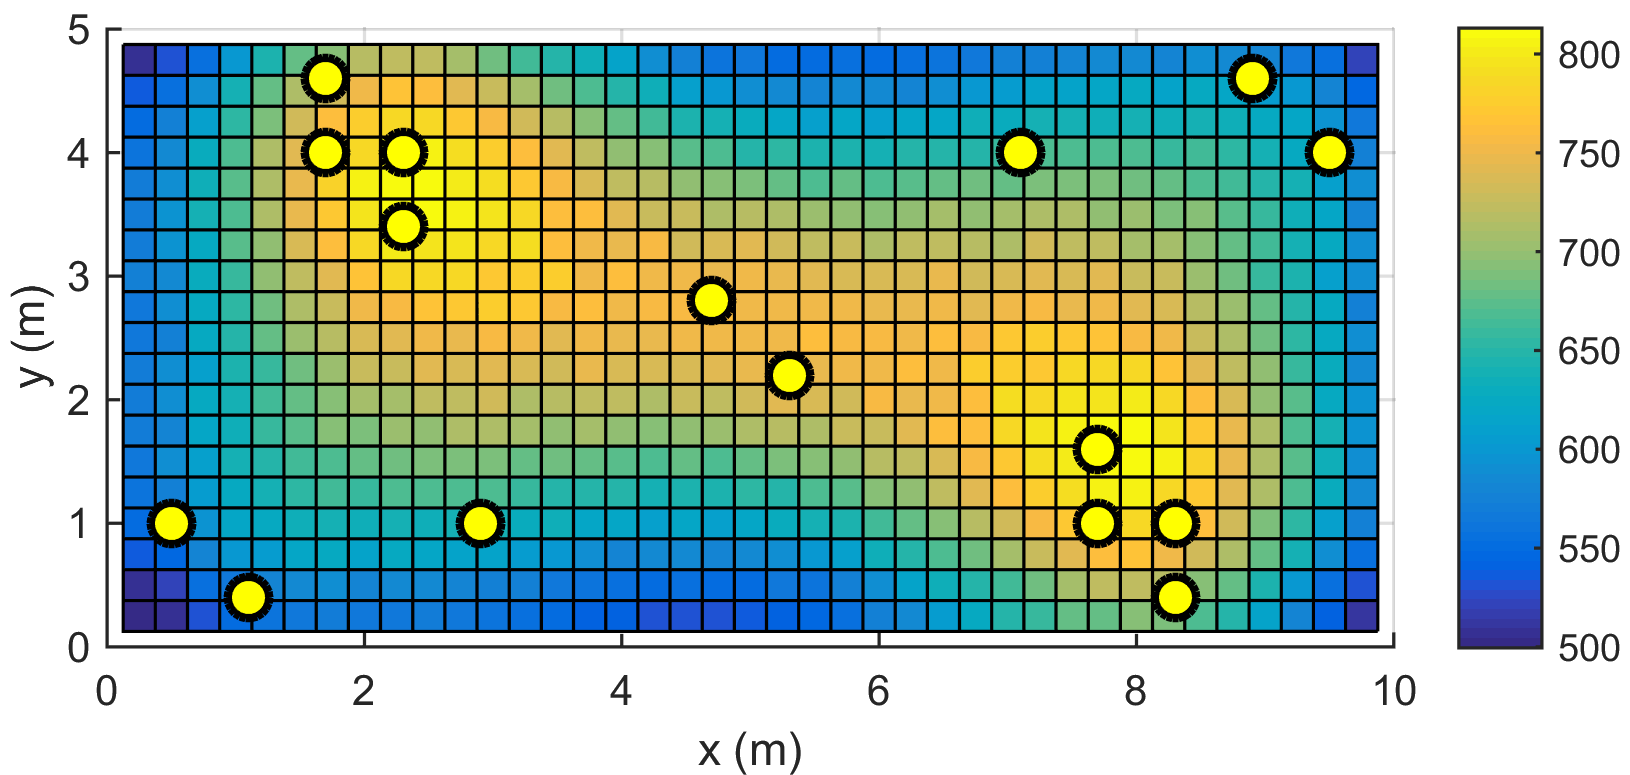
\includegraphics[width=\columnwidth]{MSTR_SLB_4x18W_5G4_Fit2_V010_S0}
  \caption{Luminaires placement with rotational symmetry}
  \label{fig:V010_S0}
\end{figure}

\begin{figure}[tb]
  \centering
  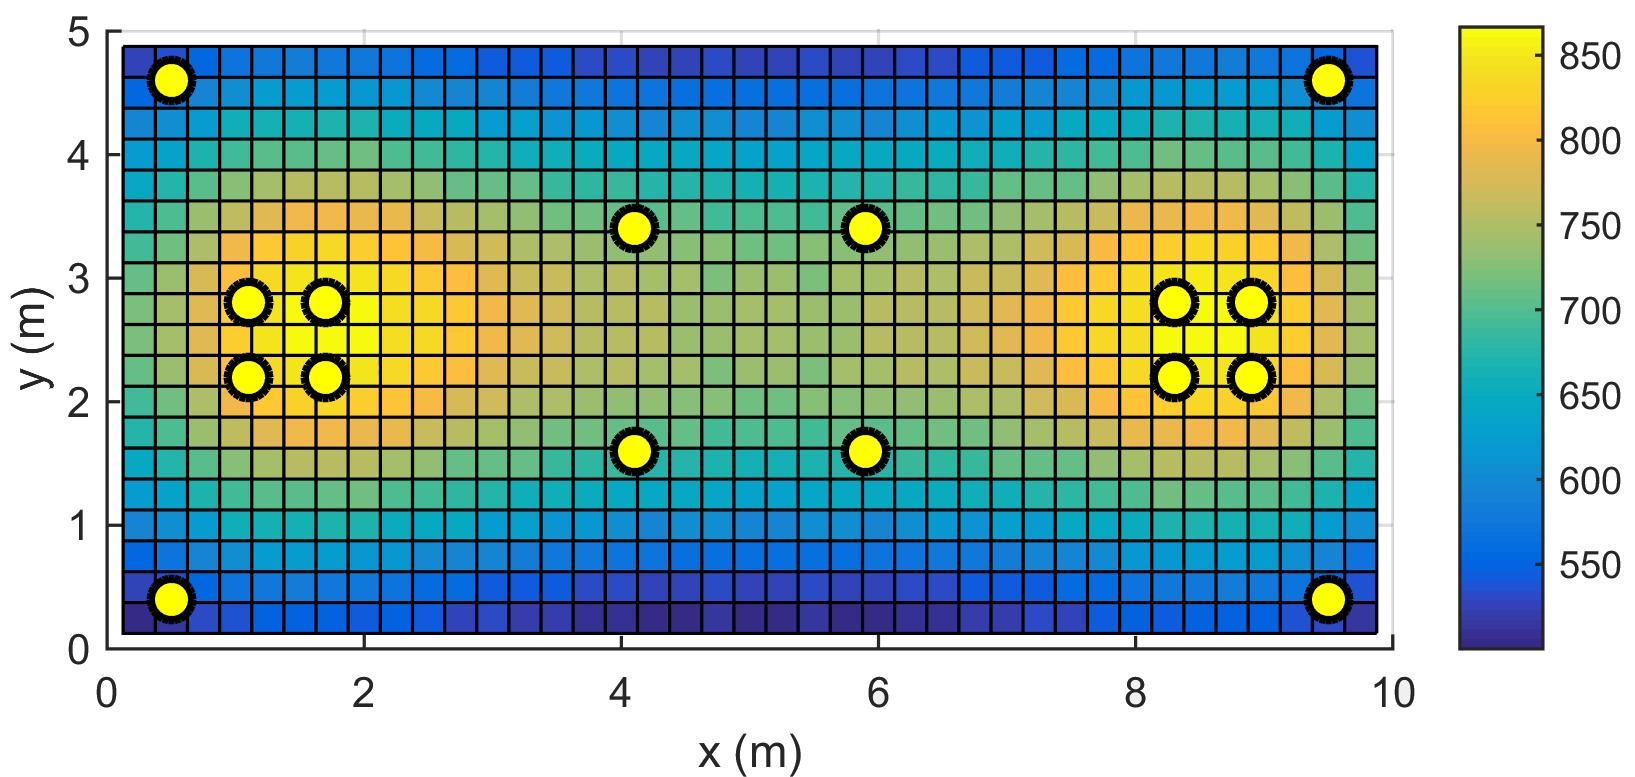
\includegraphics[width=\columnwidth]{../Vysledky/MSTR_SLB_4x18W_5G4_Fit2_V010_S1}
  \caption{Luminaires placement with mirror symmetry}
  \label{fig:V010_S1}
\end{figure}

\subsection{Different Preferences}

Results for different preference settings, i.e. preferring illuminance or preferring uniformity,can be found in Figures~\ref{fig:V010_S1_E}, \ref{fig:V010_S1_U} respectively and in Table~\ref{tab:preferences}. These results show that the parameter not being preferred was stuck at its minimal allowed value in both cases. The placement design for $\alpha = 0$ is more compressed around the longitudinal axis of the room (Figure~\ref{fig:V010_S1_E}). There is a narrow area with high illuminace that increases the resulting average illuminance. The results for $\alpha = 1$ are very similar to the results with no preferences in Figure~\ref{fig:V010_S1} and Table~\ref{tab:symmetry}. This was common to the presented type of luminous intensity distribution curve. However after comparing all three ratios R it can be seen, that the highest ratio has been obtained in the case of preferred illuminance and the lowest in the case of preferred uniformity.

\begin{table}[tb]
	\renewcommand{\arraystretch}{1.8}
	\caption{Results for different preferences}
 	\label{tab:preferences}
	\centering
  \begin{tabular}{| c | c | c |}
    \hline
    & $\alpha = 0$ & $\alpha = 1$ \\
    \hline
    $\overline{E}_{m}$ (lx) & 555 & 504 \\
    \hline
		$U_0$ ($-$)& 0.6 & 0.76 \\
    \hline
		$C$ (-) & 16 & 16 \\
	\hline
		$R$ (-) & 1.11 & 0.80 \\
  \hline
  \end{tabular}
\end{table}

\begin{figure}[tb]
  \centering
  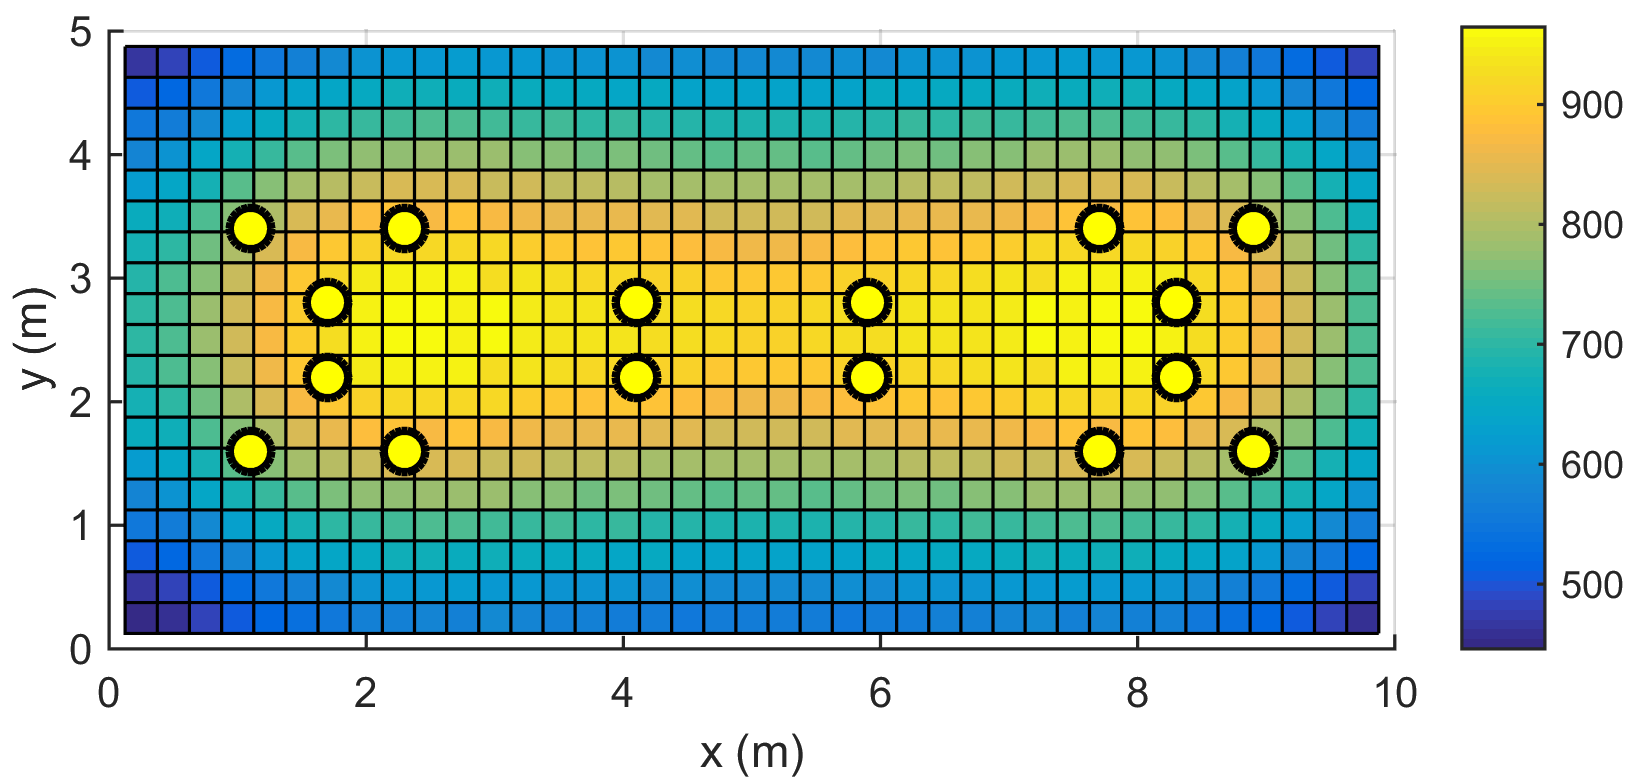
\includegraphics[width=\columnwidth]{../Vysledky/MSTR_SLB_4x18W_5G4_Fit2_E_V010_S1}
  \caption{Luminaires placement with prefered illuminance}
  \label{fig:V010_S1_E}
\end{figure}

\begin{figure}[tb]
  \centering
  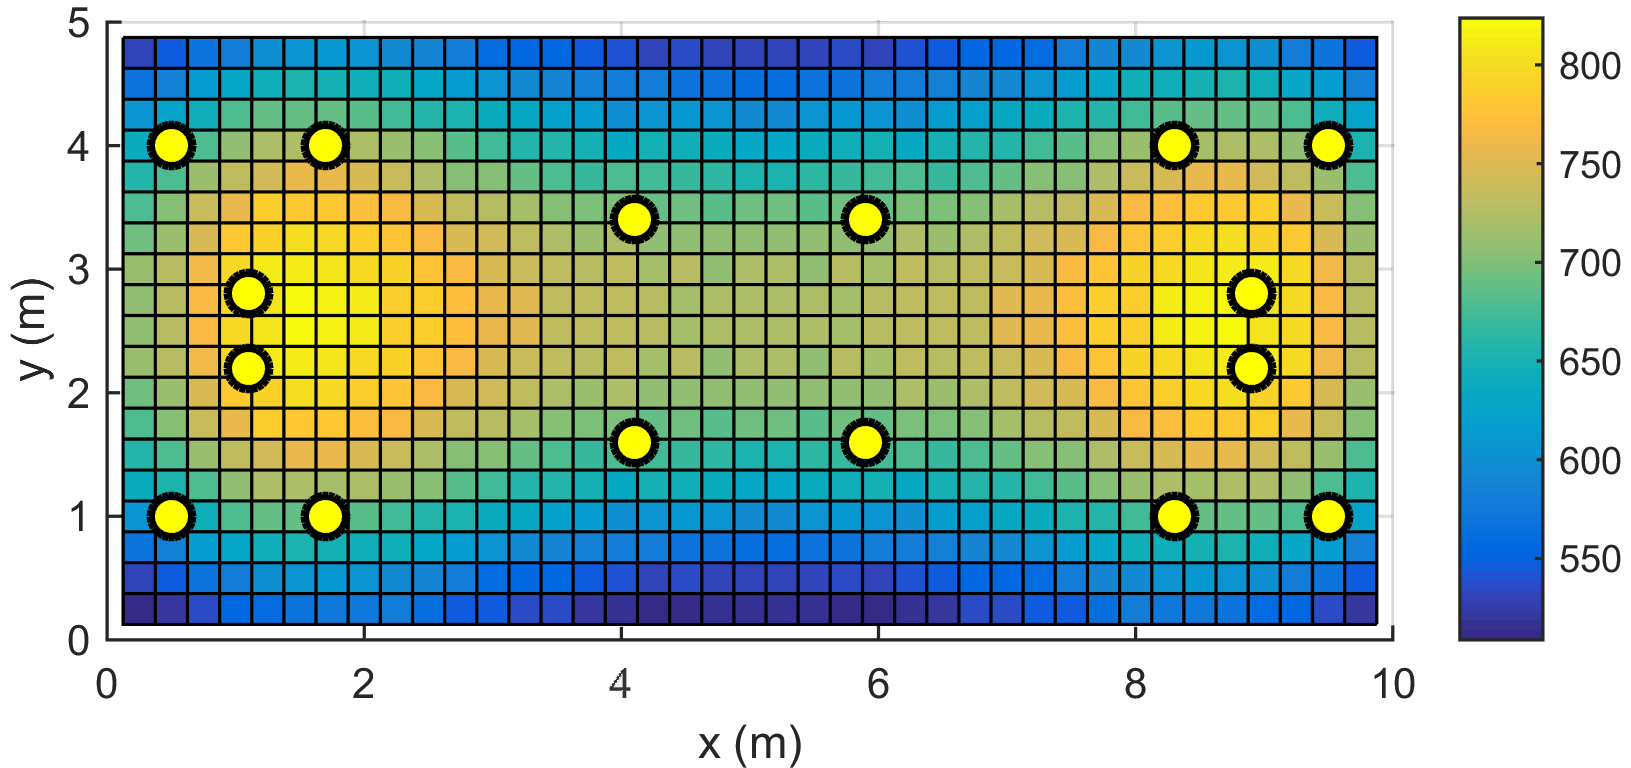
\includegraphics[width=\columnwidth]{../Vysledky/MSTR_SLB_4x18W_5G4_Fit2_U_V010_S1}
  \caption{Luminaires placement with prefered uniformity}
  \label{fig:V010_S1_U}
\end{figure}

\subsection{Without reflections}

The behavior of the GA results without calculating reflections has been tested too. The design without reflections is shown in Figure~\ref{fig:V010_S1_NoRef}. Results when reflections only of the south wall have been disabled are shown in Figure~\ref{fig:V010_S1_NoSWall}. The resulting watched values are presented in Table~\ref{tab:noRef}. The number of luminaires C is higher in these cases in comparison to the number of luminaires of the equivalent case with calculated reflections for all walls in Figure~\ref{fig:V010_S1} and Table~\ref{tab:symmetry}. It is common that the luminaires are placed closer to walls that are darker (walls not reflecting light). Luminaire distances were even smaller from the south wall compared to results of preferred uniformity. Asymmetric illuminace for symmetric luminaire placement can be seen in Figure~\ref{fig:V010_S1_NoSWall}. Both cases show that the design is clearly affected by the usage of reflections. Therefore they cannot be omitted from the algorithm.

\begin{table}[tb]
	\renewcommand{\arraystretch}{1.8}
	\caption{Results for missing reflections from any wall}
 	\label{tab:noRef}
	\centering
  \begin{tabular}{| c | c | c |}
    \hline
    & \textbf{Without walls} & \textbf{Without south wall} \\
    \hline
    $\overline{E}_{m}$ (lx) & 509 & 521 \\
    \hline
		$U_0$ ($-$)& 0.67 & 0.75 \\
    \hline
		$C$ (-) & 20 & 20 \\
	\hline
		$R$ (-) & 0.91 & 0.83 \\
  \hline
  \end{tabular}
\end{table}

\begin{figure}[tb]
  \centering
  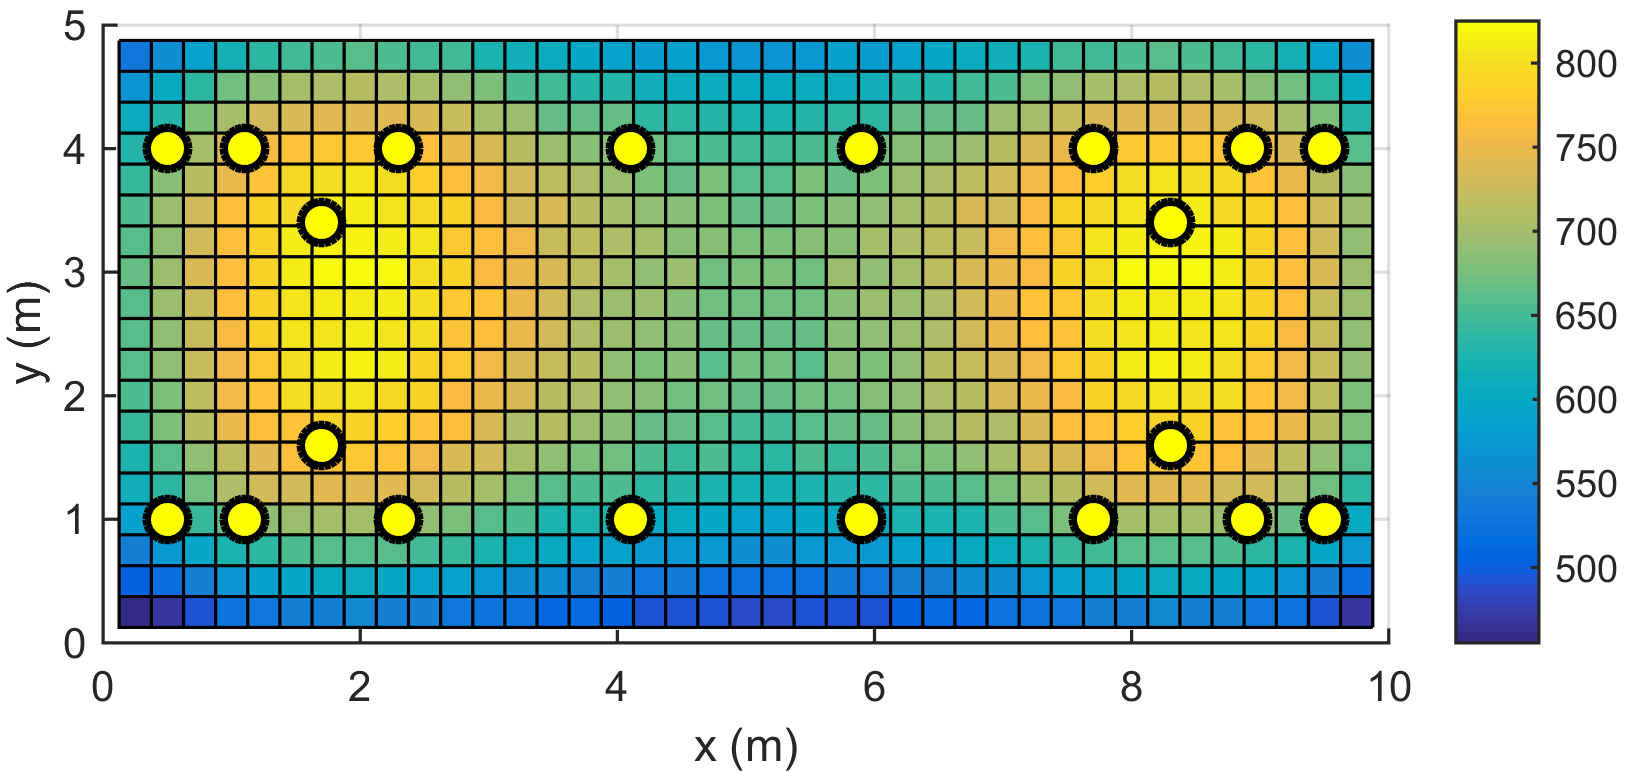
\includegraphics[width=\columnwidth]{../Vysledky/MSTR_SLB_4x18W_5G4_Fit2_NoRef_V010_S1}
  \caption{Luminaires placement without reflections from the walls and ceiling}
  \label{fig:V010_S1_NoRef}
\end{figure}

\begin{figure}[tb]
  \centering
  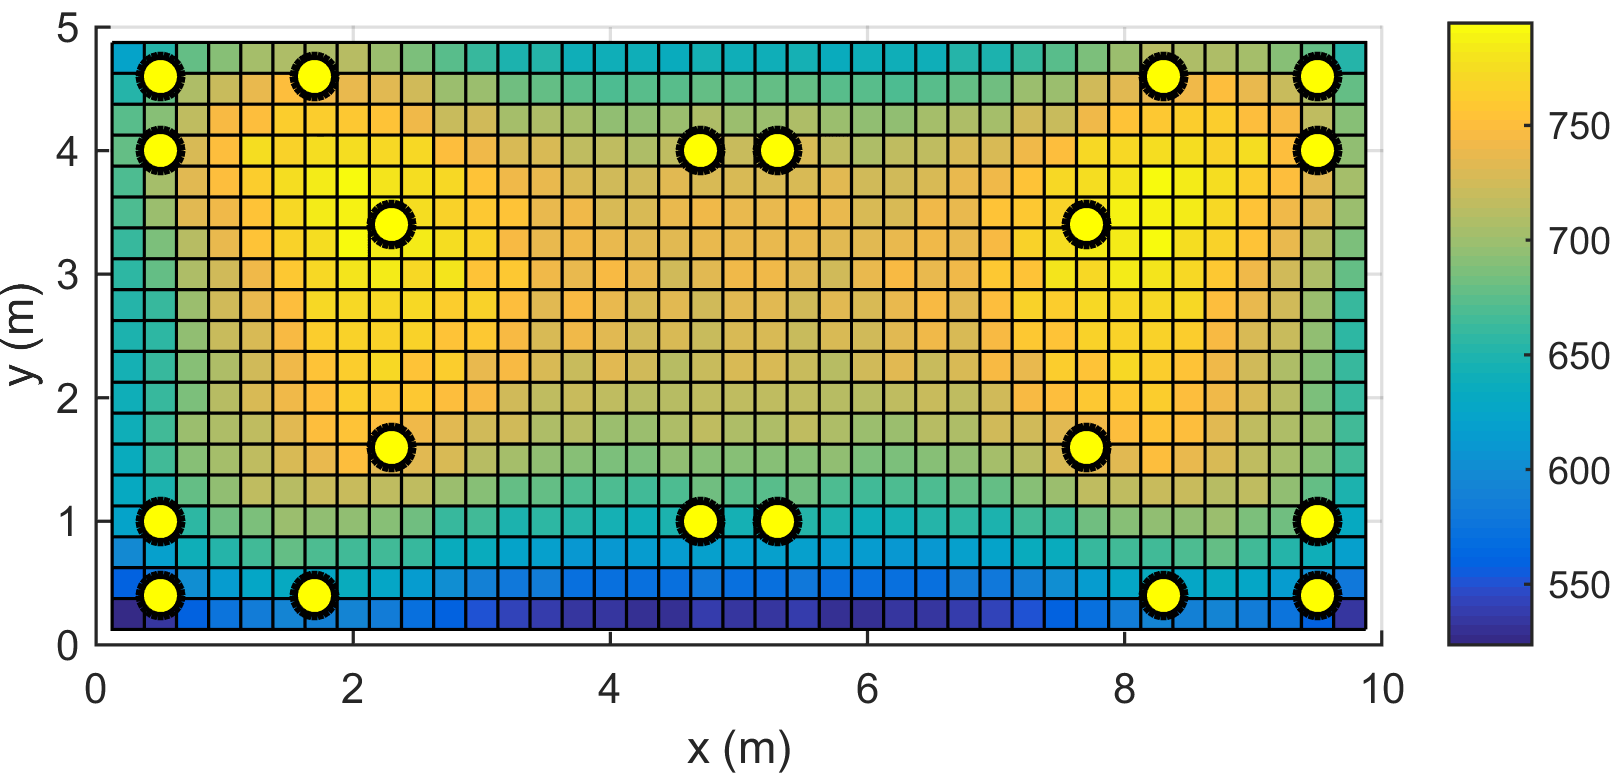
\includegraphics[width=\columnwidth]{../Vysledky/MSTR_SLB_4x18W_5G4_Fit2_NoSWall_V010_S1}
  \caption{Luminaires placement with no reflections from the south wall}
  \label{fig:V010_S1_NoSWall}
\end{figure}